\section{Direct Preference Heads}
The hypothesis underlying the Direct Preference Optimization framework of Rafailov et al. \cite{rafailov2023direct} is that a ``language model is secretly a reward model'' thereby making the purpose of Direct Preference Heads to exploit this and extract explicit reward signals without the need of an \emph{additional} reward model.

% Unlike other RLHF pipelines such as PPO \cite{schulman2017proximal}, these rewards are not used for RL fine-tuning. Instead, the DPH rewards are to be used to prune candidate generations sampled from the LM at inference time to select the candidate which aligns most with human preferences.

% This makes DPH an excellent choice for small language models which are (1) more lightweight -- and therefor can be efficiently used to generate multiple samples -- and, (2) are more prone to degradation when aligned using typical RL techniques \cite{bekbayev2023poison, bai2022training}.

\subsection{Reward Head}
% \begin{wrapfigure}{R}{5.5cm}
%     \centering
%     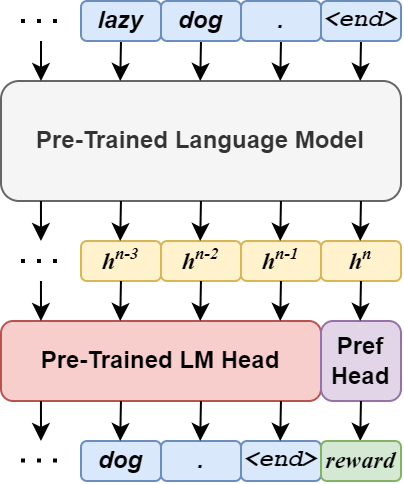
\includegraphics[width=5.5cm,trim={0 0 0 1cm}]{figures/mode_diagram.png}
%     \caption{Architecture of an LM augmented with DPH.}
% \end{wrapfigure}
To obtain the rewards from a sequence $x;y$ three components are required: an aggregated hidden state $h$ which is conditioned on the intermediate representations of the language model, a pooling function $f$ which transforms the hidden state, and a learnable vector $w_{dph}$ with the same dimension as the output of $f$. We then compute the reward $r$ as follows:
\begin{equation}
    r=f(h) \cdot w_{dph}
\end{equation}
To obtain the hidden state we take the output of the last transformer layer for the final token of the sequence, and we experiment with three choices of $f$: (1) the identity mapping following the convention established by OpenAI's GPT for sequence classification \cite{Radford2018ImprovingLU}, (2) a learnable affine projection with $\tanh$ nonlinearity following BERT's pooling function \cite{devlin2019bert}, and (3) an inverted bottleneck FFN with SwiGLU activation mirroring the FFN blocks used within the transformer backbone followed by $\tanh$ nonlinearity \cite{shazeer2020glu}.
% \begin{subequations} \label{eq:pooling_funcs}
%     \begin{alignat}{2}
%     f_{\text{GPT}}(h) &= h \\
%     f_{\text{BERT}}(h) &= \tanh{(Wx+b)} \\
%     \todo{f_{\text{SwiGLU}}(h)} &= \todo{\tanh{(W_3((W_2x + b_2)\otimes\text{SiLU}(W_1x + b_1)) + b_3)}}
%     \end{alignat}
% \end{subequations}

\subsection{Objective Function}
We formulate two novel objective functions for our method: a separable objective which maximises positive rewards and minimises negative rewards, and a contrastive objective which maximises the margin between positive and negative rewards. The loss landscapes are illustrated by Figure~\ref{fig:both_dph_loss} in the appendix.

\subsubsection{Separable DPH}
The Separable DPH loss function given by \eqref{eq:sep_dph} is a function of the preferred and dispreferred rewards $r_w,r_l$, and the label smoothing parameter $0 \leq \epsilon \leq 0.5$ which controls the reward margin.
\begin{equation} \label{eq:sep_dph}
    \mathcal{L}_\text{SepDPH}(r_w,r_l)=
    - \left[ (1-\epsilon) \log \sigma(r_w) + \epsilon\, \log \sigma(-r_w) \right]
    - \left[ \epsilon\, \log \sigma(r_l) + (1-\epsilon) \log \sigma(-r_l) \right]
\end{equation}

\begin{theorem} \label{thrm:sep_dph_convergence}
For all $\epsilon \in (0,0.5]$ the objective function $\mathcal{L}_\text{SepDPH}$ is convex and will optimize the policy $\pi_\theta$ such that the preferred rewards $r_w$ produced by the preference head converge towards $\log\tfrac{1-\epsilon}{\epsilon}$ and the dispreferred rewards $r_l$ converge to $\log\tfrac{\epsilon}{1-\epsilon}$. %\todo{When $\epsilon=0$ the objective function will never converge and gradients $\nabla_\theta \mathcal{L}_\text{SepDPH}$ will never be zero.}
\end{theorem}

This can be proven by observing the first and second partial derivatives of the loss function with respect to the rewards. The first partial derivative is equal to zero at the points $r_w=log\tfrac{1-\epsilon}{\epsilon}$ and $r_l=\log\tfrac{\epsilon}{1-\epsilon}$ respectively, and the second partial derivative is strictly positive for all values of $r_w,r_l$. A full proof is included in Appendix~\ref{sec:sep_dph_proof}.

\subsubsection{Contrastive DPH}
Like Separable DPH, the loss function for Contrastive DPH given by \eqref{eq:con_dph} is function of the preferred and dispreferred rewards $r_w,r_l$ and the label smoothing parameter $0 \leq \epsilon \leq 0.5$. This version of the loss function optimizes the \textit{relative} margin between the rewards rather than optimizing the \textit{absolute} positive and negative rewards as in Separable DPH.
\begin{equation}
    \mathcal{L}_\text{ConDPH}(r_w,r_l)=
    - (1-\epsilon) \log\sigma(r_w-r_l)
    -  \epsilon\, \log\sigma(r_l-r_w)
    \label{eq:con_dph}
\end{equation}

% \vspace{3pt}

\begin{theorem} \label{thrm:con_dph_convergence}
For all $\epsilon \in (0,0.5]$ the objective function $\mathcal{L}_\text{ConDPH}$ is convex and will optimize the policy $\pi_\theta$ such that the difference between preferred rewards $r_w$ and dispreferred rewards $r_l$ produced by the preference head will converge to a fixed margin, given by $r_{\Delta}=r_w-r_l=\log\tfrac{1-\epsilon}{\epsilon}$. %\todo{When $\epsilon=0$ the objective function will never converge and gradients $\nabla_\theta \mathcal{L}_\text{ConDPH}$ will never be zero.}
\end{theorem}

This can be proven by reparameterising the loss function such that $r_{\Delta}=r_w-r_l$ and by then considering the first and second partial derivatives with respect to this reward margin. It can be observed that the first partial derivative is equal to zero when $r_{\Delta}=\log\tfrac{1-\epsilon}{\epsilon}$, and the second partial derivative is strictly positive for all values of $r_{\Delta}$. A full proof is included in Appendix~\ref{sec:con_dph_proof}.

\subsubsection{Relation to cDPO}
The properties of both Contrastive DPH and Seperable DPH show a strong relationship with Conservative DPO: SepDPH will converge to optimal \textit{fixed reward margins} above zero for $r_w$ and below zero for $r_l$; ConDPH will converge to optimal \textit{fixed reward margins} between $r_w$ and $r_l$, and cDPO will converge to a \textit{fixed delta from the reference model} \cite{cdpo}. Like Conservative DPO, this makes both Seperable DPH and Contrastive DPH robust to preference label noise and makes training more stable than naive maximum likelihood estimation without label-smoothing.

% This establishes a strong relationship between the \textit{Contrastive DPH objective} and \textit{Conservative DPO} when label smoothing is employed, since ConDPH will converge to an optimal \textit{fixed reward margin} while cDPO will converge to a \textit{fixed delta from the reference model}. Like cDPO, this makes Contrastive DPH robust to preference label noise and will likely make training more stable \cite{cdpo}.

\subsection{Novelty over Traditional Reward Modelling}
Although similar to the reward modelling phase of an RLHF pipeline, DPH has some distinct differences which set it apart. DPH does not require an SFT sampling and human labelling stage meaning it can take advantage of pre-constructed preference datasets such as those used for DPO. Typical RLHF also requires multiple models -- a reward model, a reference model and a policy model -- while DPH requires only a single model to produce both responses and rewards. Unlike other RLHF pipelines such as PPO \cite{schulman2017proximal}, the rewards produced by DPH are not used for RL fine-tuning; instead, the DPH rewards are to be used to prune candidate generations sampled from the LM at inference time to select the candidate which aligns most with human preferences. This makes DPH an excellent choice for small language models which are (1) more lightweight -- and therefore can be efficiently used to generate multiple samples -- and, (2) are more prone to degradation when aligned using typical RL techniques \cite{bekbayev2023poison, bai2022training}.